一条指令的执行需要经过3个阶段:\textbf{{取指令、译码、执行}}{;}每个阶段都要花费一个时钟周期,如果没有采用流水线技术,那么执行N条这样的指令就需要3N个时钟周期,如下图所示。

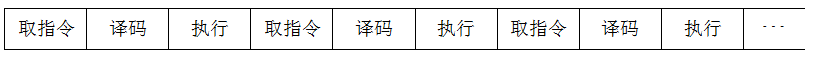
\includegraphics[width=3.12500in,height=0.22917in]{png-jpeg-pics/8A2AC62E00E6340404E548DB75815AE5.png}

当第N-2条指令在执行的时候应该对第N-1条指令进行译码,当第N-1条指令在译码时,可以将第N条指令取出来,这样就缩短了每条指令的平均执行周期。\textbf{这就是指令流水线的思想,}如下图所示。

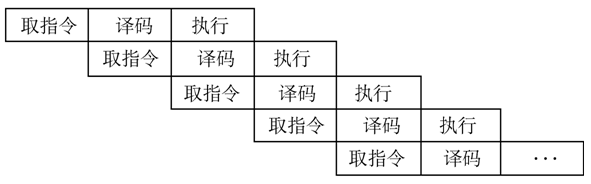
\includegraphics[width=3.33333in,height=1.04167in]{png-jpeg-pics/FF25CFF0348B51C2F179B1FBD64D1E66.png}

\textbf{当使用指令流水线时,}执行N条指令需要的时钟周期数为N+2。当N较大时,N+2远远小于3N。
